\chapter{Utilizing Onboard Compute In SteelEagle}

This chapter discusses work to replace the communications relay used in
SteelEagle to the Modal AI VOXL 2. The VOXL 2 offers significant computational
capability, allowing the execution of machine learning models.  We start by
characterizing this shift in offloading strategy in more general terms.

\section{The Computation Offload Spectrum}
\begin{figure}[htbp]
\centerline{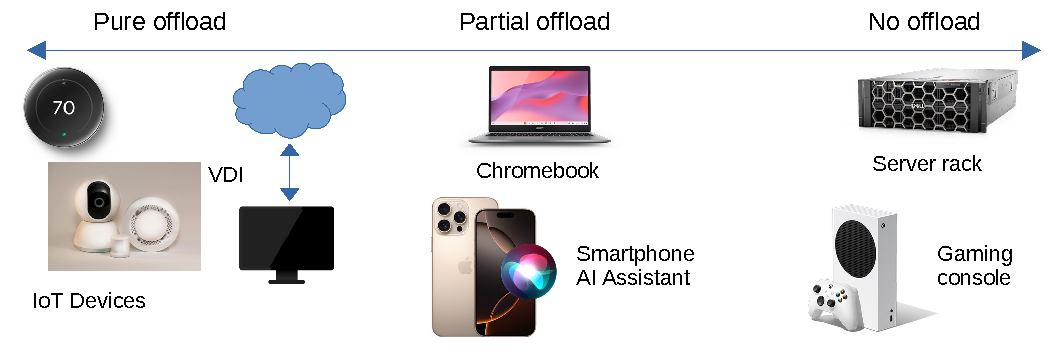
\includegraphics[width = .8\textwidth]{figs/offload-spectrum-crop.pdf}}
\caption{Devices Placed in the Computation Offloading Spectrum}
\label{fig:offload-spectrum}
\end{figure}
Devices today leverage offloading to various degrees.
\Cref{fig:offload-spectrum} shows how devices can be placed in an offloading
spectrum, with thin clients found towards the left of the spectrum and thick
clients to the right. A thin client, as opposed to a thick client, has minimal
compute and can be made smaller, lighter, and cheaper. Virtual desktop
infrastructure (VDI), for example, leverages pure offload by providing remote
access to desktops hosted on centralized servers.  This reduces the
computational demands on the client device, enabling the use of
computationally-intensive applications on weaker and older ``thin'' hardware,
reducing costs. Similarly, internet-of-things (IoT) sensors, such as video
cameras, cirumvent their limited storage and computational ability by
leveraging pure offload, transmitting their sensor streams to the cloud for
storage and analysis.

On the other end of the spectrum, we find devices such as gaming consoles,
desktop computers, and autonomous cars. Gaming consoles and desktop computers
are expected to have crisp interaction, which is not achievable by offloading
to cloud. Offloading to cloudlets, which can provide low latency, is not a
feasible option for these devices currently because of the absence of
widespread cloudlet infrastructure.  Gaming consoles and desktop computers can
provide high-levels of onboard computational power because they are not subject
to mobility constraints.  Although autonomous cars are mobile, they typically
have sufficient energy available to perform intensive onboard computations
since the majority of energy is needed to propel the car forward. They must
also perform real-time decision making reliably even in the absence of network
connectivity, which makes offloading less appealing.

In the middle of the spectrum, we find devices that perform partial offloading.
These devices have sufficient computational power to function when offloading
is unavailable or not advantageous, but they also offload computation in other
cases. Smartphone AI voice assistants such as Apple's Siri, for example,
originally offloaded all computation to the cloud. Over time, it evolved to
utilize on-device capabilities to perform simpler tasks, allowing its use in
the absence of an internet connection.  Chromebooks were designed with a focus
on the use of cloud-based services, allowing them to be fitted with lower
processing power, memory, and storage capacity compared to traditional laptops.

\subsection{How should applications decide the offloading strategy?}
\label{sec:deciding-offloading-strategy}

Choosing an offload strategy for a given application can be done based on some
key attributes that are considered important for the application:
\begin{enumerate}
    \item \textbf{Mobility requirements}: is the application subject to
        mobility constraints?
    \item \textbf{Disconnected operation}: does the application need to work reliably
        in the face of network disconnection or degradation? Is degraded operation
        acceptable during disconnected operation?
    \item \textbf{Latency requirements}: is the application latency-sensitive?
        Are there tasks that are computationally intensive but can tolerate
        high latency if a nearby cloudlet is unavailable?
    \item \textbf{Bandwidth constraints}: how much network bandwidth is
        available to the application?
    \item \textbf{Cost requirements}: is low cost for devices a priority in
        this application?
\end{enumerate}

These attributes encapsulate the benefits and limitations of offloading.
Offloading is typically only relevant for mobile devices. A mobile device that
is dependent entirely on offloading will be unable to function adequately when
offloading is impossible altogether because of network disconnection, or
impacted because of degraded network conditions, such as high latency and low
bandwidth availability. Applications that are mission-critical would be wise to
equip devices with sufficient computational resources to support an acceptable
level of function when adverse network conditions impact offloading.
Applications that are not mission-critical can rely on pure offload to benefit
from the cost savings resulting from using devices that are not required to
have significant computational resources.

Offloading allows mobile devices to achieve a much higher level of
functionality that their onboard hardware allows for. Equipping mobile devices
with the hardware needed to maintain the same level of functionality during
offload degradations reduces the benefit of offloading---the mobile device is
weighed down with the additional size and weight of more complex hardware that
remains unused when offloading is possible.

If offload degradations are infrequent, a more reasonable approach is to
utilize the inferior on-device computational resources to compute results that
are inferior according to an output-specific metric, compared to those obtained
using offloading. For predictions from a machine learning model, the metric
could be the accuracy of the prediction. In previous work, the concept of
\textit{fidelity} has been used in this context, defined as the degree to which
the results differ according to the metric \cite{noble1997}.

\subsection{The dynamic nature of partial offload}

Network conditions affect the performance of offloading, but they are dynamic
in nature. Mobile devices utilizing partial offload, then, must decide an
offloading strategy at runtime. But the decision is not binary---exclusively
using onboard compute or remote compute resources.  As
\cref{fig:offload-spectrum} shows, there is a wide range between the two ends
of the spectrum. Depending on the current network conditions, partial-offload
mobile devices can utilize a combination of onboard and remote computational
resources that results in optimal performance.

Mobile devices can achieve this through an optimal partitioning of applications
into local and remote components. Flinn et al tackled the issue of developing
applications that can support devices with different capabilities and dynamic
execution conditions with a self-tuning remote execution system. The system,
called \textit{Spectra}, continuously monitors the application's resource
supply and demand and suggests which components of an application should be
executed remotely, taking into account factors such as performance, energy
usage, and fidelity \cite{flinn2002}. This work requires the application
developer to partition the application, specifying application components
that could benefit from remote execution.

\subsection{Offloading shaping}
\label{sec:offload-shaping}

Hu et al \cite{hu2015} showed that there is value to doing additional onboard
computation when offloading, which was not originally part of the application.
The approach, called \textit{offload shaping}, attempts to conserve wireless
bandwidth and energy through the process of \textit{early discard}. The process
involves selectively sending inputs for offload computation based on an
application-specific metric of value assigned to each input.  In the case of
video analytics, for instance, onboard computation can detect blurry frames and
not transmit them to the cloudlet. Hu et al showed that object recognition does
not perform well on blurry frames, and so it is a waste of bandwidth and energy
to transmit these blurry frames to a cloudlet for computation.

\section{A Partial Offload Pipeline for SteelEagle}

SteelEagle drones can currently be placed in the ``pure offload'' part of the
spectrum in \cref{fig:offload-spectrum}, since they do not perform any on-board
computation other than the encoding of the raw camera feed to an RTSP H.264
video stream that is transmitted to a cloudlet. As discussed in
\cref{sec:deciding-offloading-strategy}, a pure offload strategy does not
support disconnected operation, and impacts the application considerably as
network conditions degrade.

\begin{figure}[htbp]
\centerline{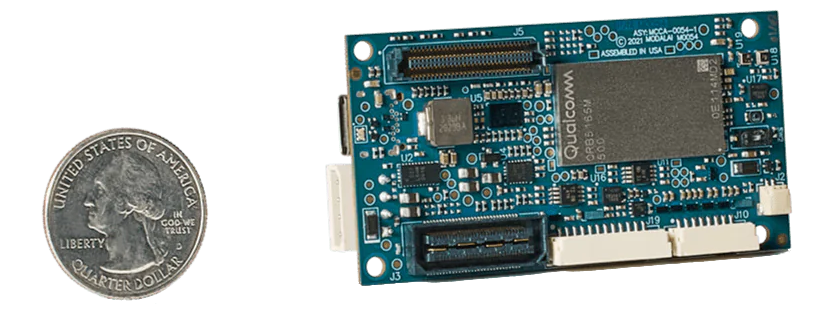
\includegraphics[width = .5\textwidth]{figs/voxl2.png}}
\caption{Modal AI VOXL 2}
\label{fig:voxl2}
\end{figure}

Replacing the Onion Omega 2 with the Modal AI VOXL 2 (\cref{fig:voxl2}) as the
communications relay in the SteelEagle pipeline will allow us to pursue a
partial offloading strategy that allows SteelEagle drones to gracefully react
to changes in network conditions. Intended for use as an AI autopilot in custom
drones, the VOXL 2 features a Qualcomm QRB5165 processor and a PX4 flight
controller. We do not utilize the PX4 flight controller on the VOXL.
\Cref{tab:voxl2-specs} provides information about the computational resources
available on the VOXL 2.

\begin{table}[htbp]
    \centering
    \begin{tabular}{@{}ll@{}}
        \toprule
        \textbf{} & \textbf{ModalAI VOXL 2}\\
        \midrule
        \textbf{Architecture} & 64-bit ARM\\
        \textbf{CPU} & Qualcomm Kyro 585 (7nm, released Dec 2019)\\
                     & 1 x 2.84 GHz high-performance core\\
                     & 3 x 2.42 GHz high performance cores\\
                     & 4 x 1.80 GHz low-performance cores\\
        \textbf{ISP} & Qualcomm Spectra 480\\
        \textbf{GPU} & Qualcomm Adreno 650, with support for OpenCL\\
        \textbf{DSP} & Qualcomm Hexagon 698\\
        \textbf{Memory} & 8 GB\\
        \textbf{Weight} & 16 grams\\
        \textbf{Power consumption} & 4-5 W under high load\\
        \textbf{Operating system} & Ubuntu 18.04\\
        \bottomrule
    \end{tabular}
    \caption{Technical specifications of the Modal AI VOXL 2 system-on-a-chip}
    \label{tab:voxl2-specs}
\end{table}

\begin{figure}[htbp]
\definecolor{observe-color}{RGB}{175,208,149}
\definecolor{orient-color}{RGB}{255, 255, 166}
\definecolor{decide-color}{RGB}{255,170,149}
\definecolor{act-color}{RGB}{224,194,205}
\centering
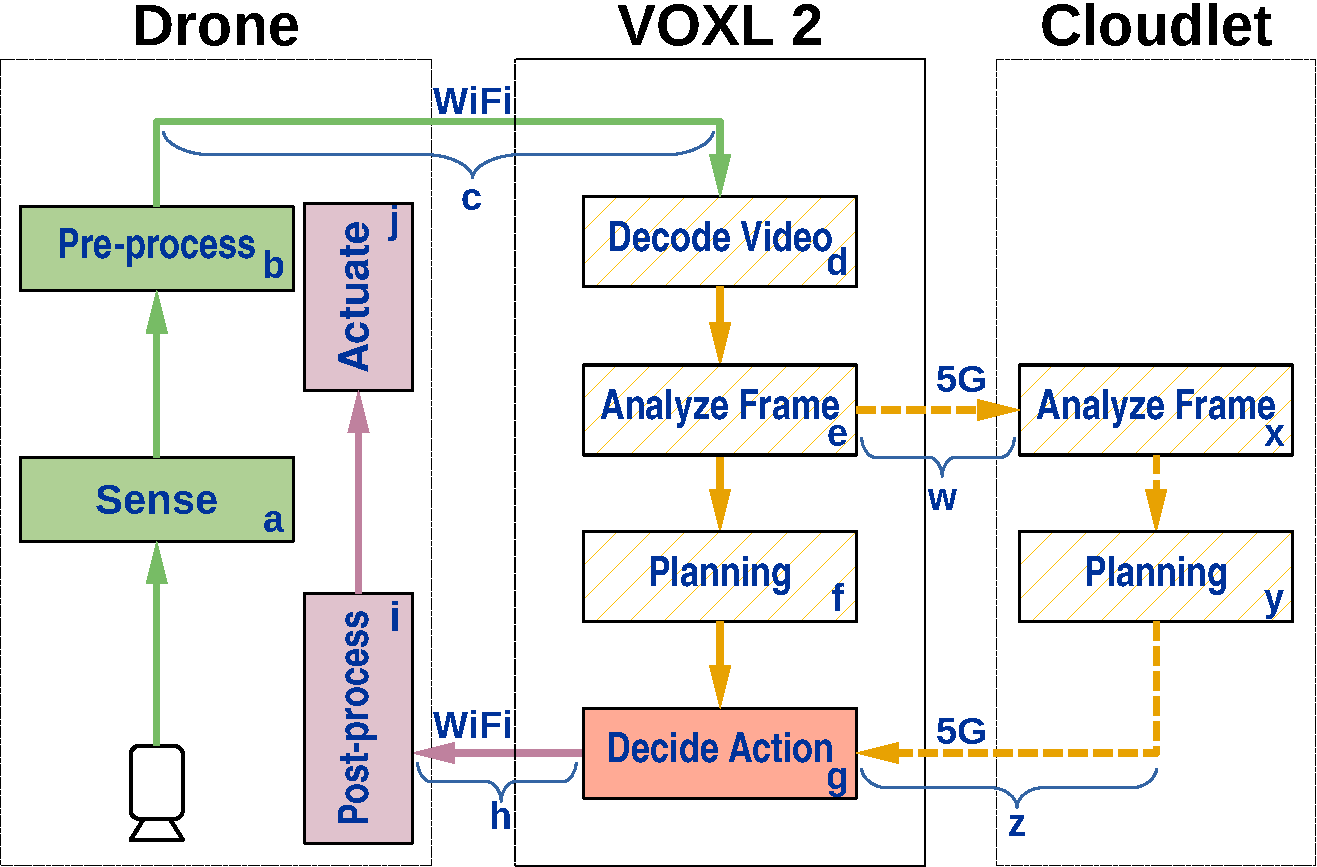
\includegraphics[width = .7\textwidth]{figs/fig-voxl-ooda-loop-crop.pdf}
\begin{comment}
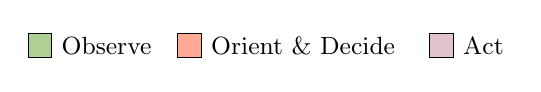
\begin{tikzpicture}
    \draw[fill=observe-color] (1.0,0) rectangle (1.3,0.3);
    \node[right] at (1.3,0.15) {\small Observe};

    \draw[fill=decide-color] (2.9,0) rectangle (3.2,0.3);
    \node[right] at (3.2,0.15) {\small Orient \& Decide};

    \draw[fill=act-color] (6.1,0) rectangle (6.4,0.3);
    \node[right] at (6.4,0.15) {\small Act};
\end{tikzpicture}
\end{comment}
\begin{tikzpicture}
    % Observe box
    \draw[fill=observe-color] (1.0,0) rectangle (1.3,0.3);
    \node[right] at (1.3,0.15) {\small Observe};

    % Orient box with yellow hatching
    \draw[fill=white, pattern=north east lines, pattern color=yellow]
        (2.9,0) rectangle (3.2,0.3);
    \node[right] at (3.2,0.15) {\small Orient};

    % Decide box
    \draw[fill=decide-color] (4.5,0) rectangle (4.8,0.3);
    \node[right] at (4.8,0.15) {\small Decide};

    % Act box
    \draw[fill=act-color] (6.2,0) rectangle (6.5,0.3);
    \node[right] at (6.5,0.15) {\small Act};
\end{tikzpicture}
\caption{Mapping the VOXL 2 pipeline to the OODA loop}
\label{fig:voxl2-ooda-loop-mapping}
\end{figure}

The VOXL 2 has support for running Google's Lite Runtime (LiteRT) machine
learning models, formely known as TensorFlow Lite (TFLite). Trained TensorFlow
and PyTorch models can be converted to LiteRT models by using techniques such
as quantization and pruning \cite{jacob2017}. Float16 quantization reduces the
floating-point precision of the model's weights to 16-bits, and full integer
quantization converts them to integers. This reduces the model's size, memory
usage and inference latency, making it more suitable for mobile device
inferencing. Float16 quantization, for instance, reduces the size of the model
by half and causes minimal loss in accuracy. However, GPU acceleration of
float16-quantized models requires half-precision floating point support (FP16)
\cite{ho2017}.

\Cref{fig:voxl2-ooda-loop-mapping} depicts the new pipeline with the VOXL 2.
In the existing SteelEagle architecture, as described in
\cref{sec:steeleagle-bg}, video decoding is performed on the cloudlet since all
video stream network packets are forwarded to the cloudlet using the Onion
Omega as a network gateway. To perform onboard computation on the VOXL 2, we
must obtain individual frames from the drone's video stream.  This requires
decoding the H.264 video stream on the VOXL 2. The Orient phase begins after
the frames are decoded.  The VOXL pipeline has an inner and outer Orient loop:
\begin{itemize}
    \item \textbf{Inner loop}: Corresponds to components Orient$_e$ and
        Orient$_f$, which involve analysis of the decoded frame and planning
        on the VOXL
    \item \textbf{Outer loop}: Corresponds to components Orient$_w$ through
        Orient$_z$. Involves offloaded analysis of the decoded frame and
        planning on the cloudlet
\end{itemize}

The outer loop involves offloading to the cloudlet, which incurs latency and
transmission delay to and from the cloudlet. The cloudlet, being a stationary
device, can run more accurate analysis and planning phases in less time.

To conserve bandwidth, the outer loop is not always exercised.  The pipeline
can leverage offload shaping techniques (\cref{sec:offload-shaping}) to
determine if the frame should be discarded. Then, a remote execution system,
such as the one developed by Flinn et al \cite{flinn2002}, can determine if
processing should be offloaded. Once frame processing is complete, the pipeline
determines whether any drone actuation needs to be performed, and generates the
corresponding command.

\subsection{Onboard Computation Design}

\begin{figure}[htbp]
\centering
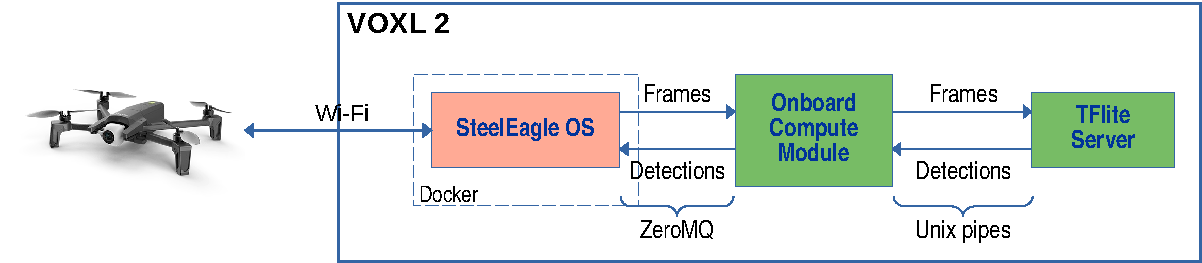
\includegraphics[width = .9\textwidth]{figs/onboard-design-crop.pdf}
\begin{captext}
Components in red are developed in Python, and components in green in C++
\end{captext}
\caption{VOXL 2 Onboard Computation Pipeline}
\label{fig:voxl2-onboard-pipeline}
\end{figure}

The VOXL 2 supports the Open Computing Language (OpenCL) standard, which
assists in writing parallel programs which leverage its hardware accelerators,
including its GPU. The VOXL 2 ships with a software suite that includes various
programs designed to be run as \texttt{systemd} services. One of these
programs, VOXL TFlite Server, performs hardware-accelerated machine learning
inference. The inputs and outputs of the programs are sent through an
inter-process communication library called \texttt{libmodalpipe}, which uses
Unix pipes. \texttt{libmodalpipe} includes data structures that represent data
items such as camera image metadata and the results of inference. For example,
\texttt{camera\_image\_metadata\_t} specifies image metadata such as width,
height, size and format of the image, and \texttt{ai\_detection\_t} includes
information relevant to object detection models, such as detected classes,
confidence levels, and bounding boxes.

VOXL TFlite Server is designed to take the drone's camera data continuously as
input through a Unix pipe and output detections through another Unix pipe. Any
service interesting in consuming the inference results can register as a client
to the output pipe. We can utilize this framework to perform onboard inference,
publishing frames requiring inference to a pipe configured as input to VOXL
TFLite Server.

The VOXL software ecosystem is targeted for C/C++ programs. However, the
SteelEagle pipeline is currently developed in Python. As a result, a C++ proxy
is required that can receive frames from the SteelEagle program and forward
them to the VOXL TFLite Server for inference.  As
\cref{fig:voxl2-onboard-pipeline} shows, an onboard compute module was
developed that communicates with SteelEagle using the ZeroMQ messaging library,
listening for inference requests. ZeroMQ has bindings available for popular
programming languages, making it suitable for this use case. A SteelEagle stub
provides a convenience API that generates a \texttt{protobuf} message that is
sent to the onboard compute module. The \texttt{protobuf} message includes the
contents of the frame as an RGB image along with frame metadata such as width
and height. The onboard compute client generates the
\texttt{camera\_image\_metadata\_t} structure that VOXL TFLite Server expects,
and sends it to its input pipe along with the frame data.

Once the VOXL TFLite Server receives an input, it publishes one
\texttt{ai\_detection\_t} data structure to the output pipe for each detection
on a given frame. There is no metadata published that specifies the number of
detections to expect. This works well if a consumer wants a live stream of
object detections. However, in our case, we only want to reply to the
SteelEagle program once we receive all detections for a given frame. To achieve
this, the VOXL TFLite Server program was modified to send a delimiter
\texttt{ai\_detection\_t} data structure once all the detections have been sent
for a given frame. Once this delimiter is received, the onboard compute module
adds all the detections to a single \texttt{protobuf} message, and sends it
back to the SteelEagle program.

\subsection{OODA Loop of VOXL 2 SteelEagle Pipeline}

Using the terminology from \cref{fig:voxl2-ooda-loop-mapping}, we consider the
performance of each component of the VOXL pipeline.

\subsubsection*{Observe$_{ab}$}

The Observe$_{ab}$ component of the OODA loop in the new pipeline is the same as in
the case of the Onion Omega (\cref{sec:onion-observe-ab}), including on-drone
sensing and pre-processing, which involves generation of an RTSP H.264 video
stream from the drone camera's raw video frames. We use the same drone,
the Parrot Anafi, for the VOXL pipeline. As before, this component has a mean
of 253 ms, with a standard deviation of 12 ms, and a p99 of 277 ms.

\subsubsection*{Observe$_{c}$}

Observe$_c$ involves a short Wi-Fi segment from the drone to the VOXL 2. Since
the VOXL 2 is mere centimeters away from the drone, this component is
negligible.

\begin{comment}
\Cref{fig:voxl2-decoding-performance} shows the latency measurements. The
latency distribution has a mean of 262 ms, with a standard deviation of 10.5 ms
and a p99 of 282 ms. This is comparable to the Observe$_{ab}$ measurements from
the Onion Omega pipeline.
\end{comment}

\subsubsection*{Orient+Decide$_{d}$}

\begin{figure}[htbp]
    \centering
    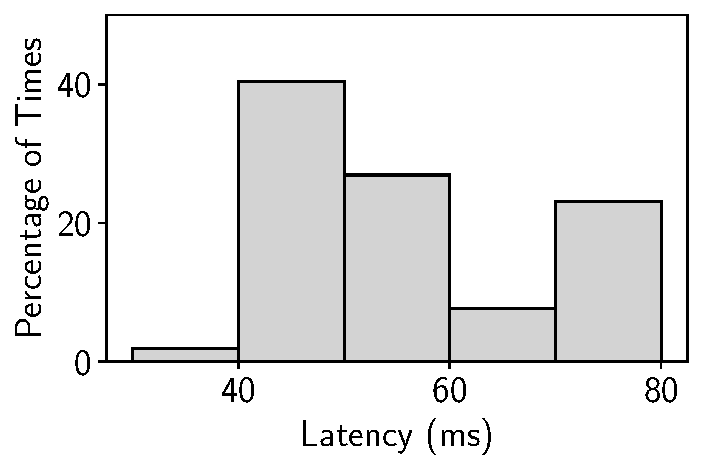
\includegraphics[width = .4\textwidth]{figs/voxl-decoding-time.pdf}\\
\small{Mean: 54.84$\pm$11.59~ms\; p99: 76.47~ms}\\
\caption{Orient+Decide$_d$ Measurements}
\label{fig:voxl2-decoding-latency}
\end{figure}

Orient+Decide$_d$ involves the decoding of the RTSP video stream generated
by the drone. \Cref{fig:voxl2-decoding-latency} shows the measurements of
the video decoding. The latency distribution has a mean of 55 ms, with a
standard deviation of 11.6 ms, and a p99 of 76.5 ms.

\subsubsection*{Orient+Decide$_{e}$}

\begin{figure}[htbp]
    \centering
    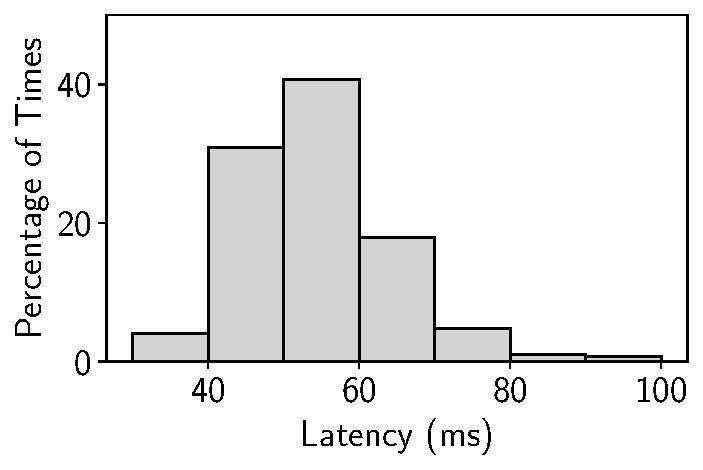
\includegraphics[width = .4\textwidth]{figs/voxl-5g-latency.pdf}\\
\small{Mean: 37.52$\pm$10.09~ms\; p99: 59.24~ms}\\
\caption{Orient+Decide$_e$ Measurements}
\label{fig:voxl2-5g-latency}
\end{figure}

Orient+Decide$_e$ is incurred when the remote execution system decides to
offload computation, and involves a 5G segment from the VOXL 2 to the cloudlet.

\subsubsection*{Orient+Decide$_{f}$}

\begin{figure}[htbp]
\centerline{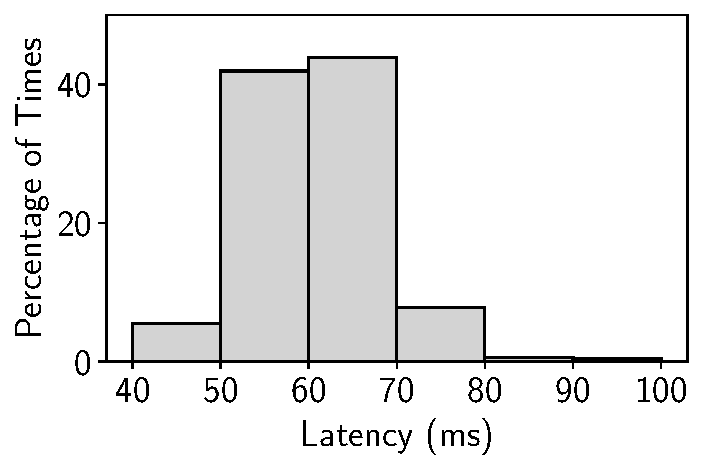
\includegraphics[width = 0.5\textwidth]{figs/onboard-inference-hist.pdf}}
\centering
Mean: 60.5$\pm$6.77~ms\; p99: 77.5~ms\\
\caption{Onboard inference on the VOXL 2 using a Float16-quantized YOLOv5 model}
\label{fig:voxl2-inference-hist}
\end{figure}

Orient+Decide$_f$ corresponds to Stage 2 and Stage 3 of the Onion Omega pipeline, discussed in \cref{sec:onion-orient-decide-d}. \Cref{fig:voxl2-inference-hist} shows measurements for running a machine learning model on the VOXL. We use a float16-quantized YOLOv5 model for inference, which is used for detecting objects. We obtain a mean latency of 60.5 ms, with a standard deviation of 6.77 ms and a p99 of 77.5 ms.

\subsubsection*{Act$_{g}$}

Act$_g$ involves a 5G segment from the cloudlet to the drone via the VOXL 2 when offloading to the cloudlet. In the case of the onboard pipeline, only a Wi-Fi segment is needed.

\subsubsection*{Act$_{hi}$}

Act$_{hi}$ is the same as Act$_{fg}$ in the Onion Omega pipeline, discussed in \cref{sec:onion-act-fg}, involving drone post-processing and actuation. For the actuation of the Parrot Anafi drone's gimbal, it has a mean of 173 ms and a standard deviation of 15 ms.

\subsection{Latency of VOXL 2 Offload Pipeline}

In the VOXL pipeline, frames are decoded on the VOXL instead of the cloudlet.
This means that if the remote execution system decides to offload computation
to the cloudlet, it must send individual frames to the cloudlet. This increases
bandwidth requirements substantially. Previously, a bandwidth of 5 Mbps was
sufficient to send the video stream to the cloudlet. Individual 720p frames
average about 180 KB when encoded as JPEG, requiring a bandwidth of 43.2 Mbps
to send 30 frames per second.  As \cref{tab:voxl2-offload-performance} shows,
the VOXL 2 does not have sufficient bandwidth to sustain this frame rate.
Reducing frame size allows us to achieve this frame rate.

\begin{table}[htbp]
    \centering
    \begin{tabular}{llll}
        \toprule
        \textbf{Frame details} & \textbf{Frame size (KB)} & \textbf{Avg. Latency (ms)} & \textbf{Achievable FPS}\\
        \midrule
        720p & 180 & 934$\pm$\small{30.47} & 12.58\\
        720p, 80\% JPG quality  & 98 & 600$\pm$\small{65.76} &28.63\\
        720p, 70\% JPG quality & 79 & 304$\pm$\small{12.82} & 29.95\\
        360p & 79 & 307$\pm$\small{20.60}  &29.89 \\
        360p, 80\% JPG quality & 38 &288$\pm$\small{13.96} & 29.89\\
        360p, 70\% JPG quality & 31 & 286$\pm$\small{17.26} & 29.85\\
        \bottomrule
\end{tabular}
\caption{Offloading Performance on the VOXL 2}
\label{tab:voxl2-offload-performance}
\end{table}
